% Template for ICIP-2019 paper; to be used with:
%          spconf.sty  - ICASSP/ICIP LaTeX style file, and
%          IEEEbib.bst - IEEE bibliography style file.
% --------------------------------------------------------------------------
\documentclass{article}
\usepackage{spconf,amsmath,graphicx}

%%%% my use package


\usepackage{cite}
\usepackage{amsmath,amssymb,amsfonts}
\usepackage{algorithmic}
\usepackage{graphicx,color}
\usepackage{textcomp}
\usepackage{bbm}
\usepackage{bm}
\usepackage{caption}
\usepackage{graphicx, subfig}
\usepackage{stfloats}

% Example definitions.
% --------------------
\def\x{{\mathbf x}}
\def\L{{\cal L}}

% Title.
% ------
%\title{L-SNet: Combine Localisation and Segmentation by ROI Recalibration  }
\title{supplementary material} 
% Single address.
% ---------------
\name{Paper number 2430}
  
\address{}
%
% For example:
% ------------
%\address{School\\
%	Department\\
%	Address}
%
% Two addresses (uncomment and modify for two-address case).
% ----------------------------------------------------------
%\twoauthors
%  {A. Author-one, B. Author-two\sthanks{Thanks to XYZ agency for funding.}}
%	{School A-B\\
%	Department A-B\\
%	Address A-B}
%  {C. Author-three, D. Author-four\sthanks{The fourth author performed the work
%	while at ...}}
%	{School C-D\\
%	Department C-D\\
%	Address C-D}
%
\begin{document}
%\ninept
%
\maketitle
%
\begin{figure*}[hb]
    \centering
    \resizebox{\textwidth}{!}{
    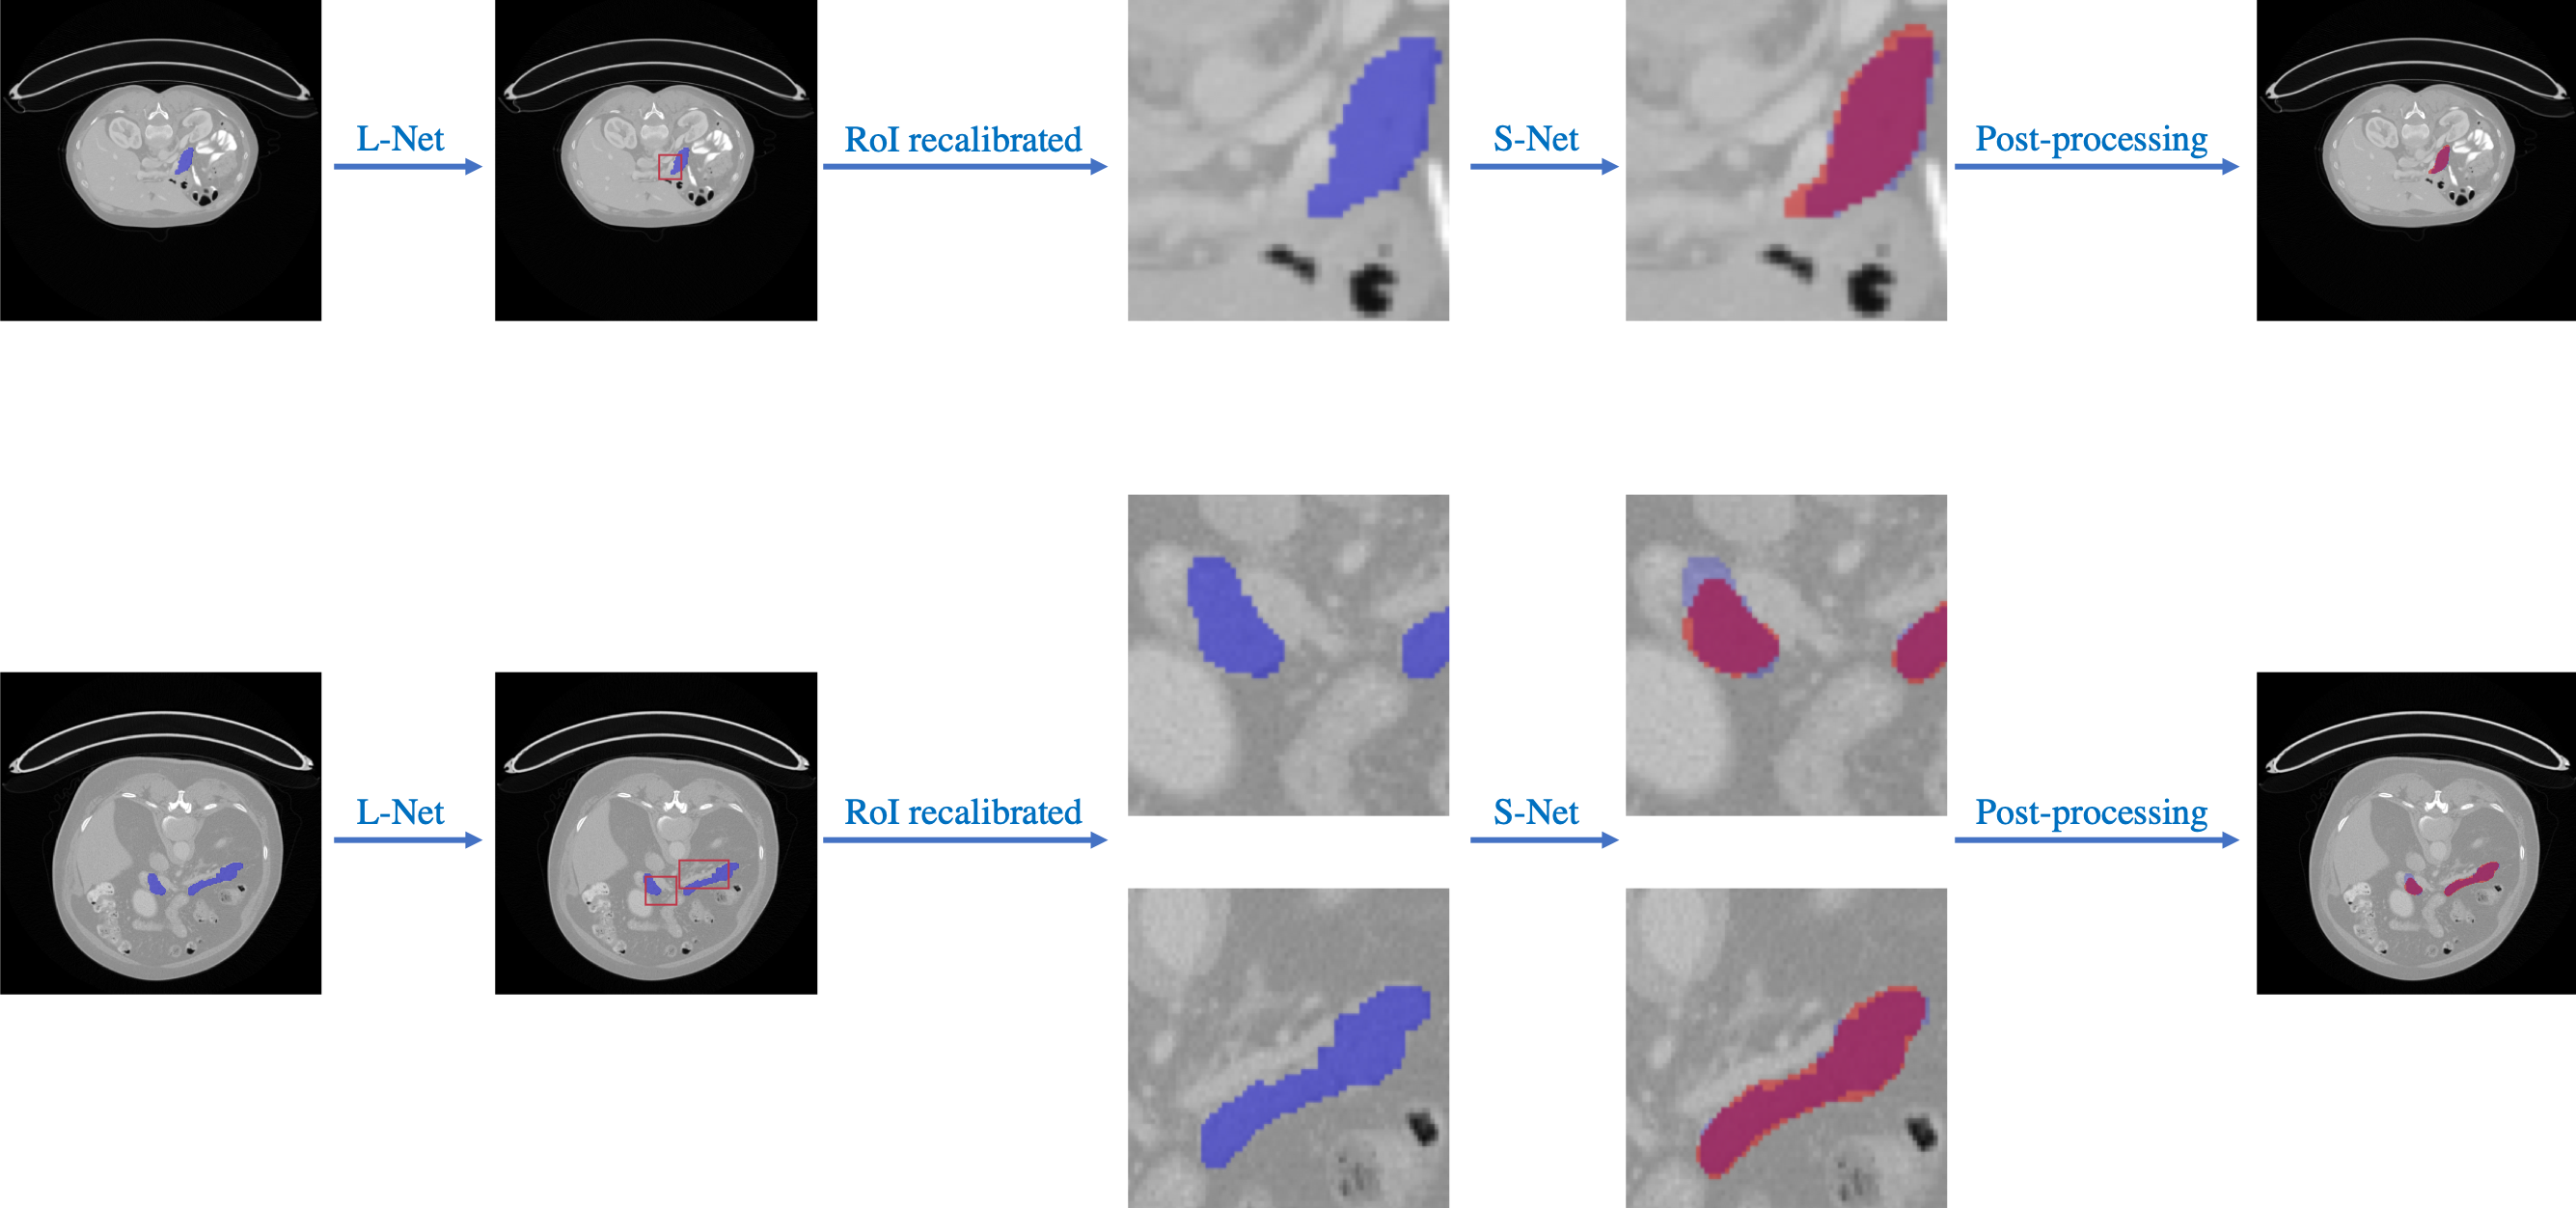
\includegraphics{s1.png}
    }
    \caption{
    Visualization of L-SNet's workflow to perform medical image segmentation, which is illustrated by two samples. The ground truth areas are shown in purple; the predicted areas are shown in pink. RoIs located by L-Net and padded with extra pixels are bounded by red boxes.}
    \label{fig:s1}
\end{figure*}

To illustrate the L-SNet's prediction process vividly, we take two samples (a trivial one and a complex one), pass them through L-SNet, and present their intermediate results (see Fig.\ref{fig:s1}).
%To further detail the inference process described in the main content: firstly, LNet locates all potential RoIs on the input image ($2_{nd}$ column); secondly, each predicted and located RoI on the source image is recalibrated by RR module into an image with a pre-defined shape (together with its ground truth mask) through affine transformation and bilinear interpolation sampling ($3_{rd}$ column); the fine segmentation results is shown in $4_{th}$ column; finally, the post-preprocessing maps the masks segmented by S-Net to their original positions and scales on the source image (last column). Noticeably, if there is multiple RoIs located by L-Net, the fine segmentation is performed on each located RoIs separately. \par


\begin{figure*}[ht]
    \centering
    \resizebox{\textwidth}{!}{
    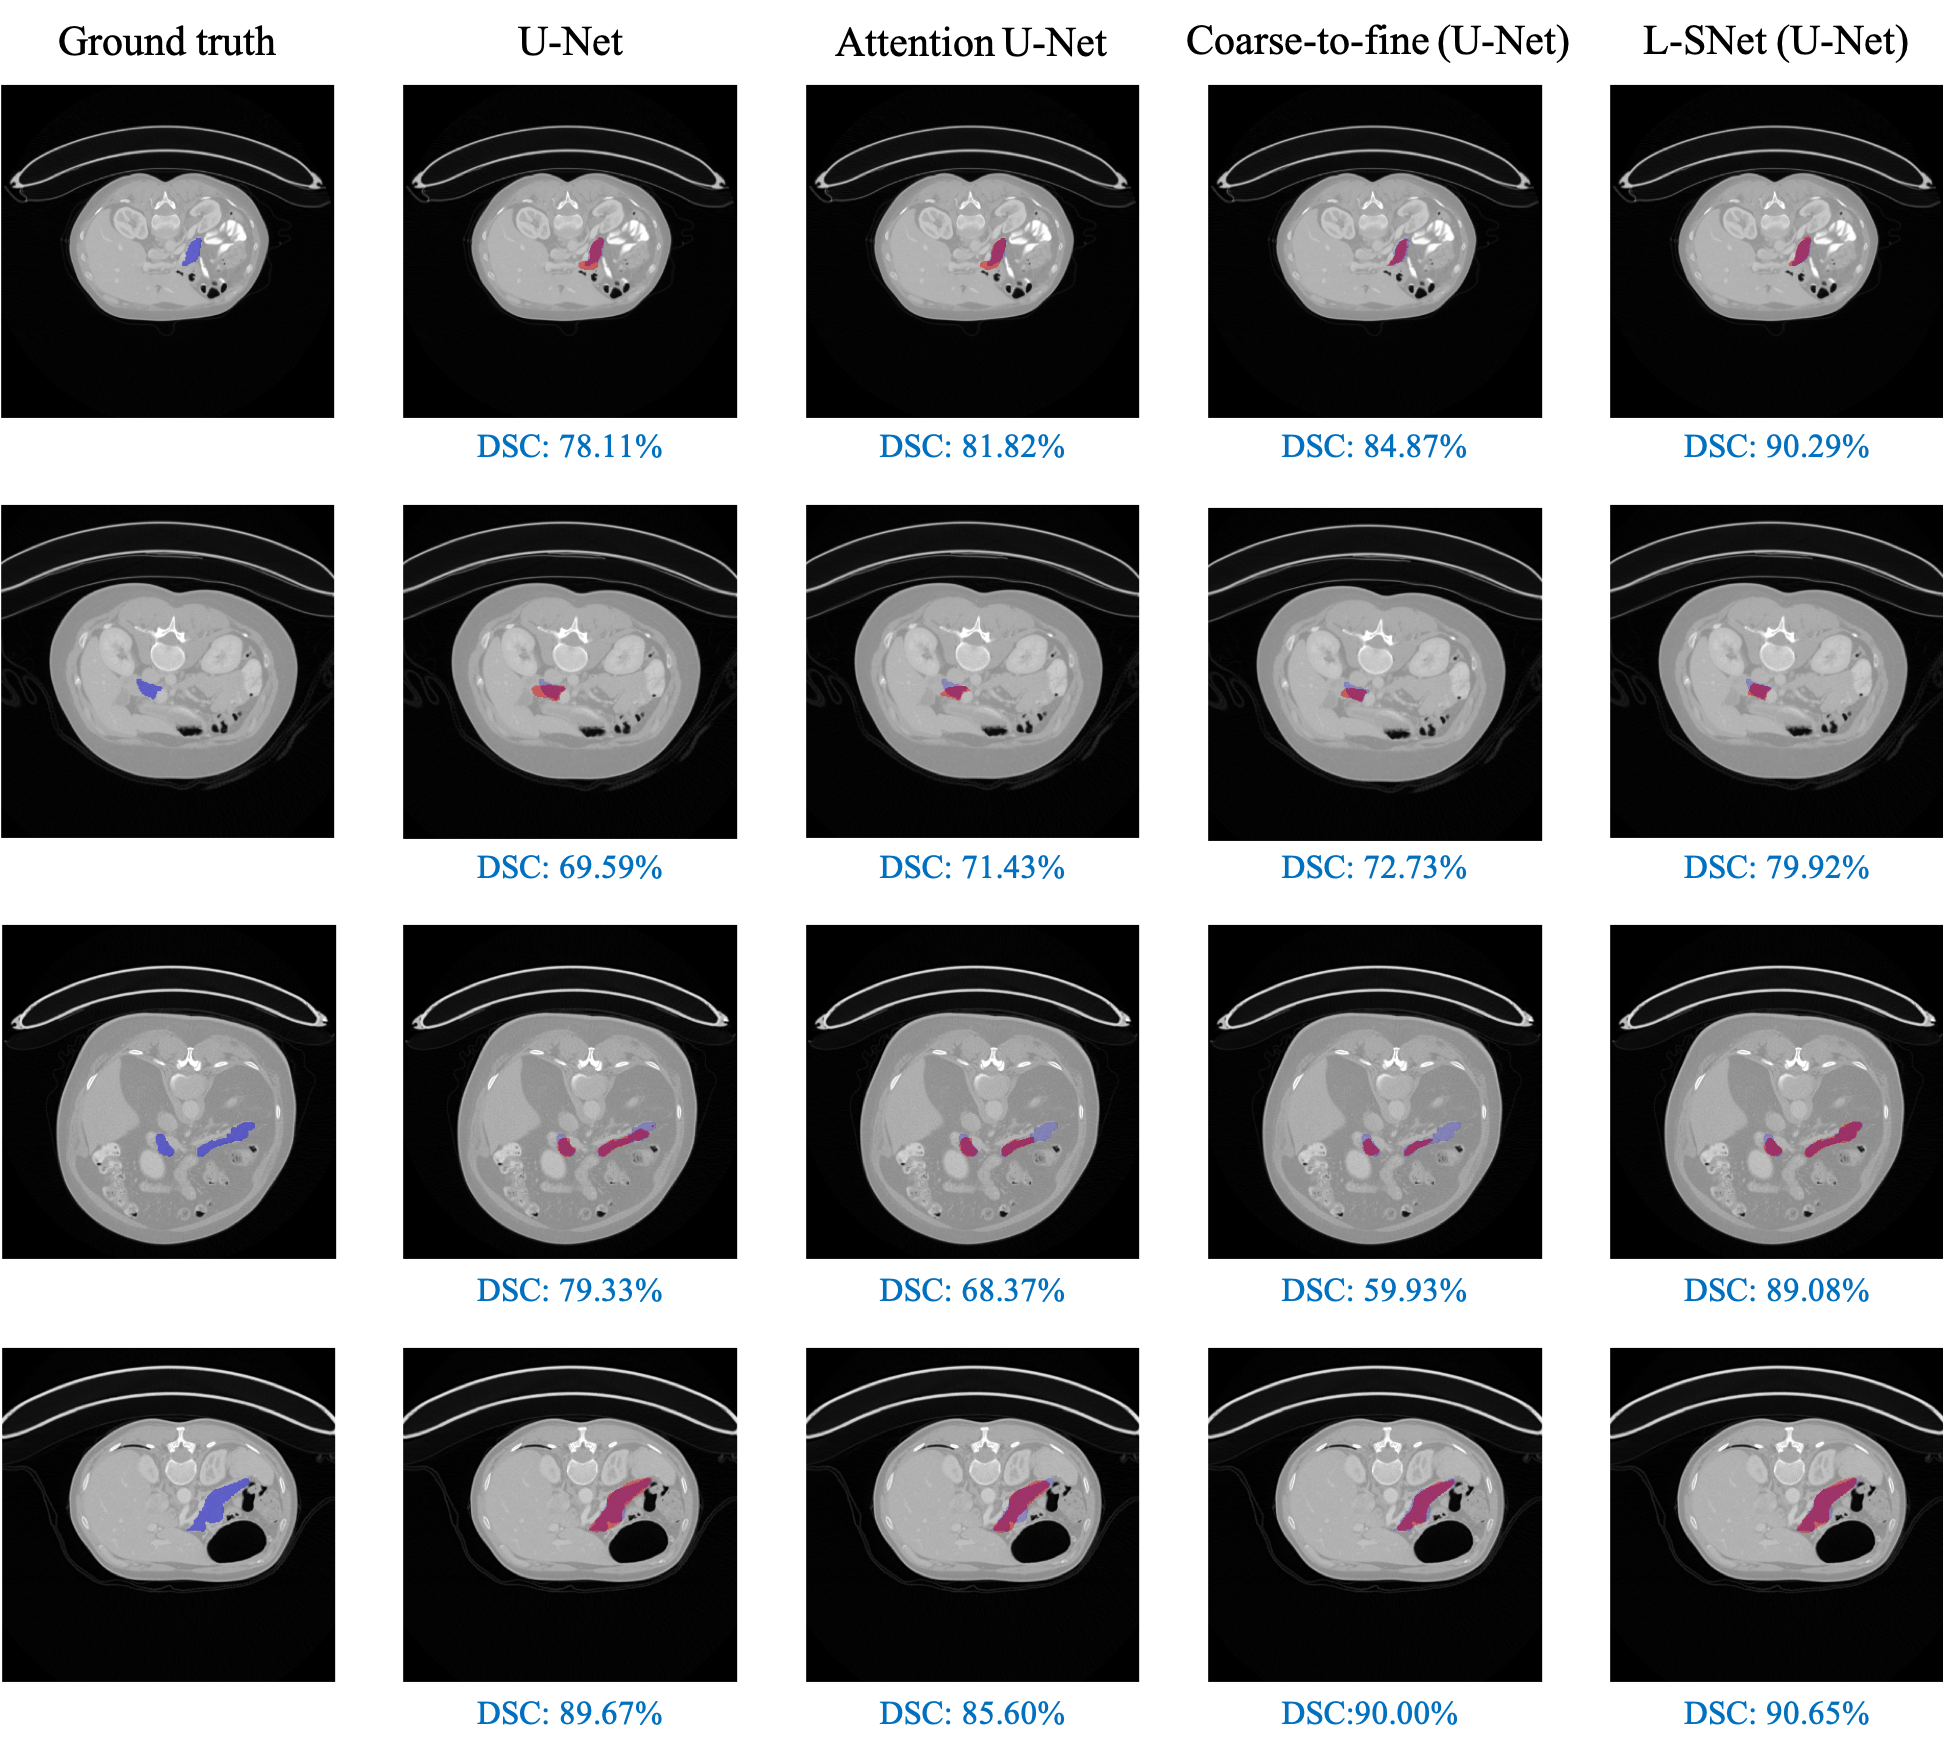
\includegraphics{s2.png}
    }
    \caption{
    Segmentation results of four samples are compared among our L-SNet and other three proposed models. The first two samples are with small scale RoIs; the third sample is with multiple RoIs; the last sample has an RoI with a larger scale. Each prediction is displayed with its segmentation result and with DSC score located below (in percentage).}
    \label{fig:s2}
\end{figure*}

%It can be observed (Fig.\ref{fig:s2}) that L-SNet outperforms all other models on DSC despite 

Fig.\ref{fig:s2} displays the segmentation performance comparison of four samples among different models.
\end{document}
